This chapter describes a methodology for directly measuring SAVAT for a pair of instructions in a system. The goal is to measure the EM emanations side-channel signal (or another type of side channel signal) created by executing instruction A vs executing instruction B (i.e. $\textrm{SAVAT}(A,B)$). A naive approach measures the signals for A and B separately, then computes the area (total amplitude difference over time) between the signal curves for A and B. Unfortunately, this naive approach has a very large measurement error. First, the single-instruction signal difference is much smaller than the overall signal generated by the execution that surrounds the instruction under examination. Complex processors heavily optimize the scheduling and execution of instructions, so determining the times where the test instructions A or B are actually active would be problematic.
Computing a small difference between two large signals is subject to huge relative error because the measurement error for each signal is proportional to the signal's overall value, i.e. the difference between signals might be dominated by measurement errors in the two measurements. Second, the computed $A - B$ signal is affected by imperfect alignment of the two signals in time. Other instructions must be present around A and B to make the measurement practical (to trigger the measurement, setup the registers and memory used by instructions A and B, etc.), and so noise and other unrelated components of the received signal obfuscate the signal components created by the A and B instructions themselves. Third, this approach requires recording many samples of the two signals (to enable accurate subtraction) over a very short period of time (the duration of a single instruction). Even the most sophisticated ($>$\$200,000 cost) instruments provide only 10-20 samples per clock cycle in modern multi-GHz processors. Equipment capable of measuring the low amplitude $a(t)$ and $b(t)$ signals at greater than 10G samples/sec (as required to test a processor using a GHz clock) is prohibitively expensive or non-existent. The naive approach for measuring an A/B SAVAT which is subject to the aforementioned problems is illustrated in Figure~\ref{NaiveMeasurement}: execute a program fragment that performs instruction/event A and record the side channel signal, then execute an identical program fragment but now with instruction/event B instead of A, record the side channel signal again, then align the two signal curves in time and compute the area between the two curves.

\begin{figure}[thb]
\centering
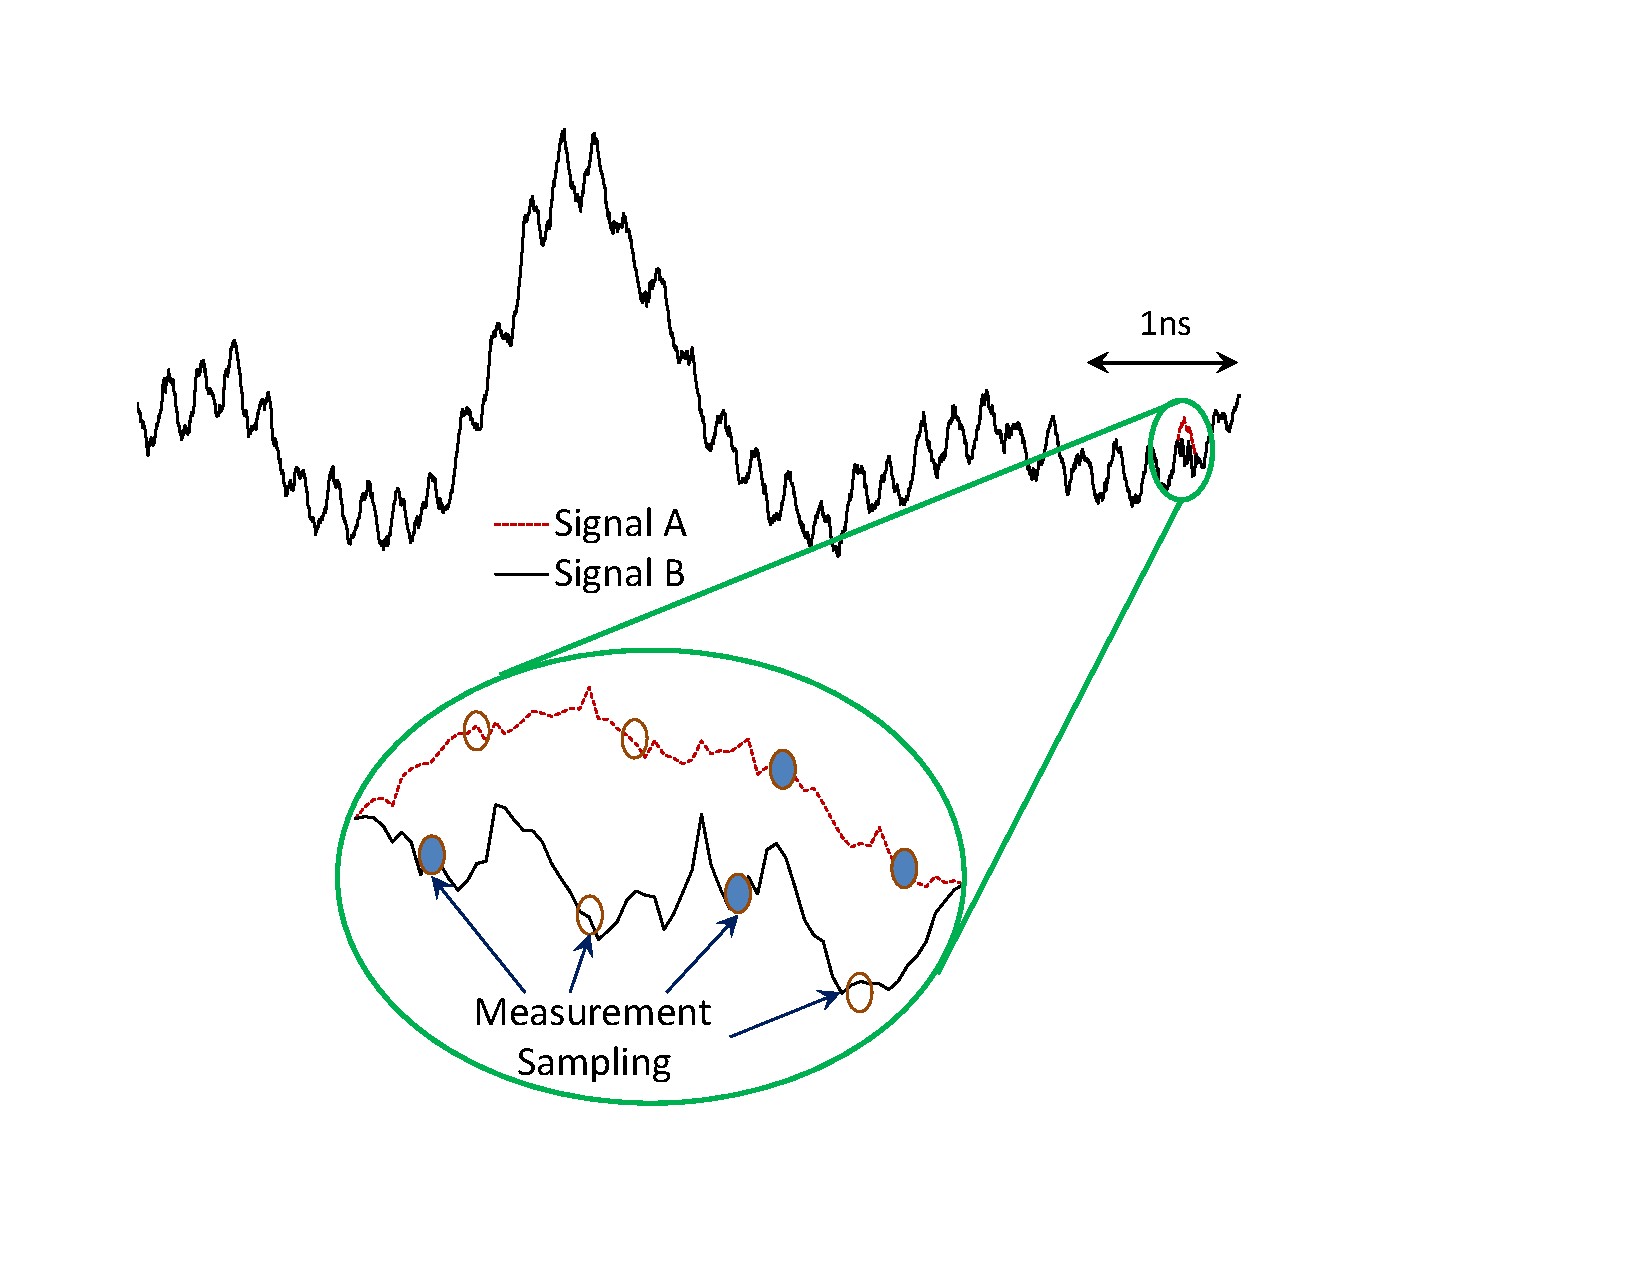
\includegraphics[trim=0.8in 1.1in 2.7in 0.8in,clip,width=5in]{../savat_final/Drawing/NaiveMeasurement.pdf}
\caption{A naive approach for measuring SAVAT.}
\label{NaiveMeasurement}
\end{figure}

To overcome these problems, our methodology employs microbenchmarks carefully constructed so that any signal due to differences between the A and B instructions is localized in frequency (Figure~\ref{PeriodicSignal}b), whereas the naive approach attempts to localize this difference in time in separate A and B signals (Figure~\ref{NaiveMeasurement}). The new A and B combined signal is constructed by having the computer system alternate between the two instructions/events (A and B) many times per second as shown in Figure~\ref{PeriodicSignal}b. This alternation generates a periodic signal at the alternation frequency that corresponds to the overall difference between the individual signals. This periodic signal can then be filtered to reject other frequencies including the noise and the uninteresting signals they carry, and the filtered signal's magnitude can then be measured. For EM emanations, power, sound, etc., this filtering and measurement can be done very precisely using a spectrum analyzer. The spectrum obtained in this way measures the difference in signal strength between A and B instructions/events over a unit time (e.g. a second), and overcomes all of the problems with the naive measurement because (1) the measured A/B difference signal accumulates over many A/B differences over this one second, effectively amplifying the signal and suppressing noise (the instrument only needs to be sensitive enough to measure the one-second total, we can still compute the single-instruction/event SAVAT by dividing the measured signal by the number of A/B instances that occur each second), (2) the difference between A and B side channel signals is directly measured, without the relative-error problem present when measuring A and B signals separately, and (3) the signal is measured at the alternation frequency, which can be adjusted in software by changing the number of A and B events per iteration of the alternation loop, so we can easily bring that frequency within the measurement range of commercially available instruments. We also have the freedom to select a frequency with relatively little noise - an important consideration for EM emanation side channels where direct collection of A and B side channel signals is subject not only to measurement error but also to noise from various radio signals. Also, while the A/B difference signal occurs at the greatly attenuated high frequencies in the naive measurement,  in this new methodology the A/B difference signal occurs at a single, known, easier-to-measure, low frequency. 

\begin{figure*}[htb]
\centering
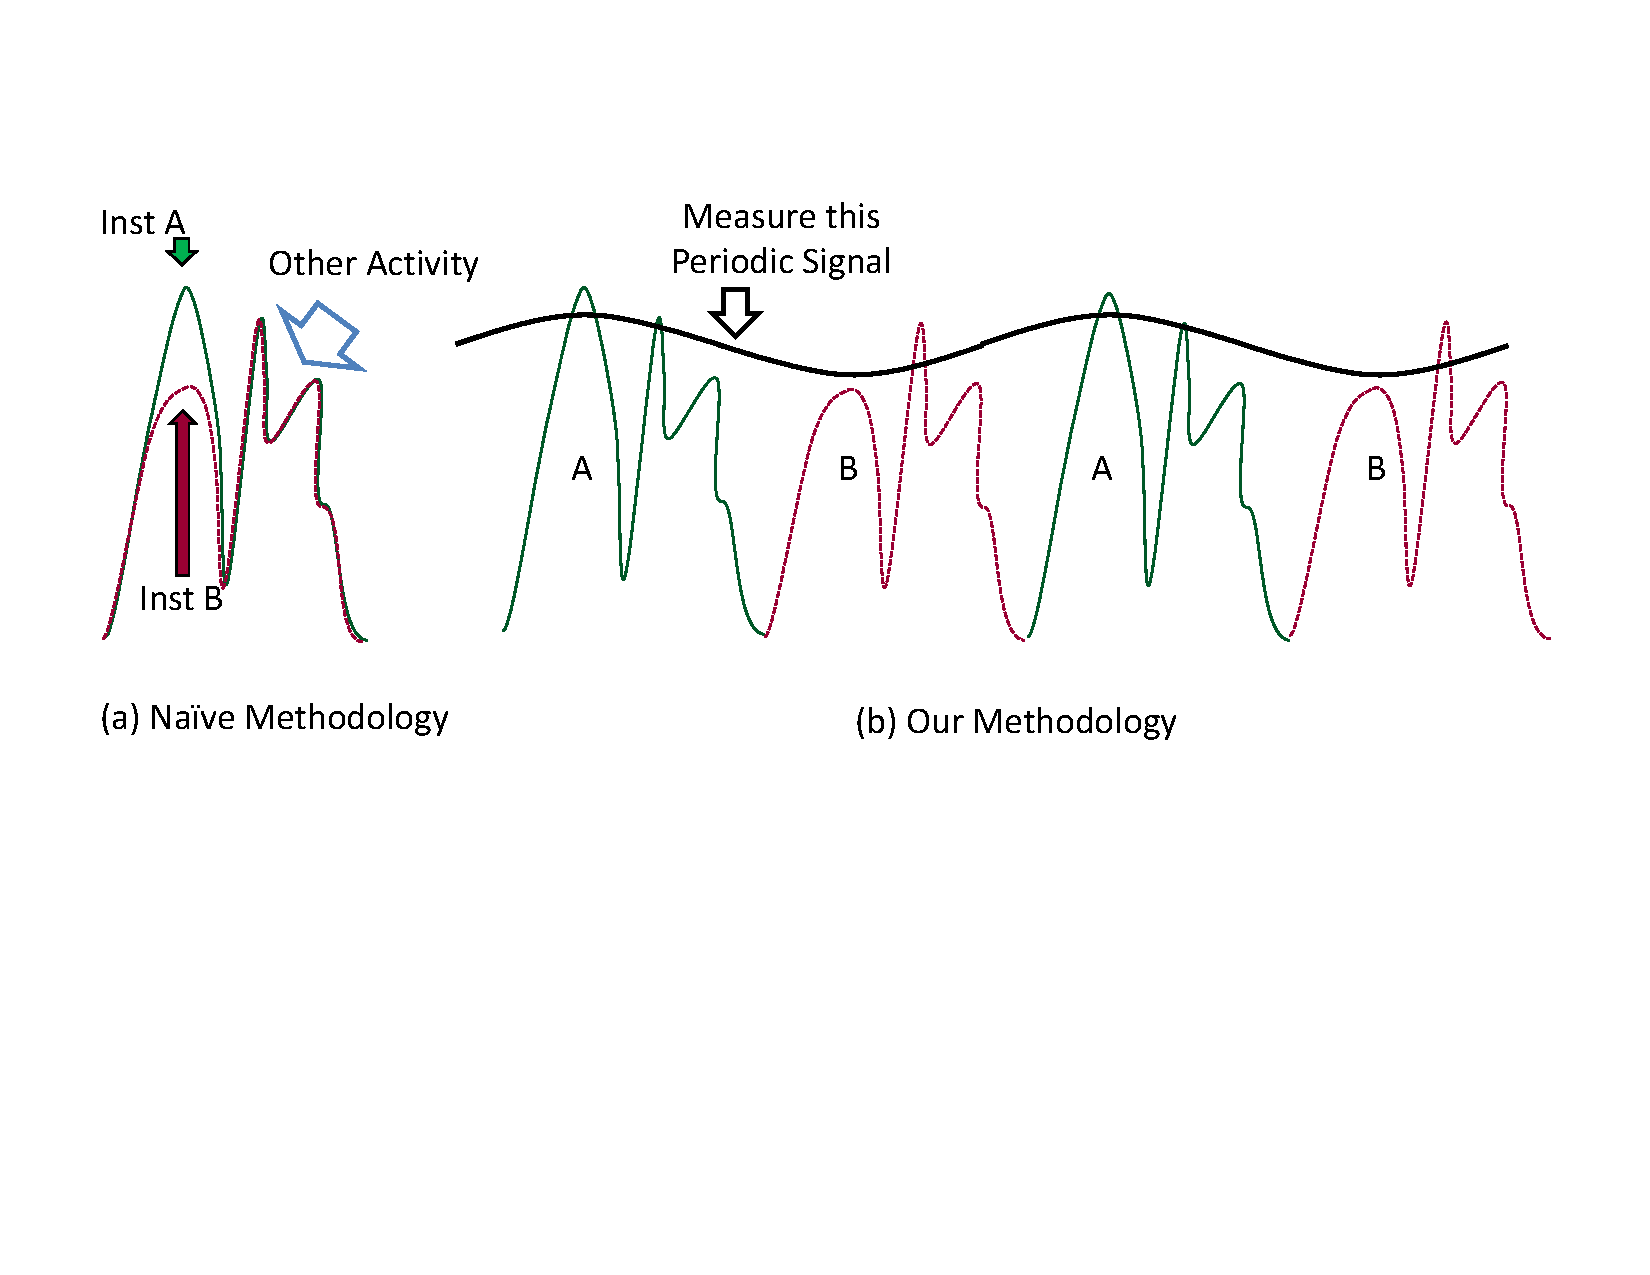
\includegraphics[trim=0.6in 3.5in 0.6in 1.3in,clip,width=6in]{../savat_final/Drawing/PeriodicSignal.pdf}
\caption{Our methodology measures the (a) signal difference by (b) alternating the signals then filtering and measuring the resulting periodic signal at the alternation frequency.}
\label{PeriodicSignal}
\end{figure*}



\begin{figure}[htb]
  \centering
\lstset{language=C++,basicstyle=\ttfamily\small,numbers=left}\lstset{escapeinside={/*@}{@*/}}
\begin{lstlisting}[frame=none,xleftmargin=30pt]
while(1){/*@\label{BegInfLoop}@*/
  // Do some instances of the A inst/event /*@\label{BegLoopA}@*/
  for(i=0;i<n_inst;i++){
    ptr1=(ptr1&~mask)|((ptr1+offset)&mask);/*@\label{UpdAddrA}@*/
    // The A-instruction, e.g. a load
    value=*ptr1;/*@\label{TestInstA}@*/
  }/*@\label{EndLoopA}@*/
  // Do some instances of the B inst/event /*@\label{BegLoopB}@*/
  for(i=0;i<n_inst;i++){
    ptr2=(ptr2&~mask)|((ptr2+offset)&mask);/*@\label{UpdAddrB}@*/
    // The B-instruction, e.g. a store
    *ptr2=value;/*@\label{TestInstB}@*/
  }/*@\label{EndLoopB}@*/
}
\end{lstlisting}
\caption{The A/B alternation pseudo-code.}\label{pseudocode}
\end{figure}

The overall structure of the code used in the measurement methodology is shown in Figure~\ref{pseudocode}. Lines \ref{BegLoopA} through \ref{EndLoopA} execute \texttt{n\_inst} instances of the A instruction/event, and then lines \ref{BegLoopB} through \ref{EndLoopB} execute the same number of instances of the B instruction. Thus lines \ref{BegLoopA} through \ref{EndLoopB} represent one A/B alternation, and this alternation is repeated (line \ref{BegInfLoop}) until the measurement of the side channel signal is complete. The value of \texttt{n\_inst} allows us to control the number of alternations per second, and we select a value that produces the desired alternation frequency for our measurements. For a given desired repetition period $T_{alt}$ corresponding to one iteration of the outer loop, $T_{alt}$ can be directly measured using counters available through processor instructions (e.g. the x86 \texttt{rdtsc} instruction) or the operating system (e.g. the Windows API \texttt{QueryPerformanceCounter()} function).  For example, increasing \texttt{n\_inst} increases the time required to execute one iteration of the outer loop ($T_{alt}$).

The benchmarks generate controllable emanations at frequency ($f_{alt} = 1/T_{alt}$) as shown in Figure~\ref{Fig:Carrier}. Intuitively we expect differences between the A and B instructions to appear at the frequency $f_{alt} = 1/T_{alt}$. More analysis is required to derive the exact relationship between the spectral power $P(f_{alt})$ (observed at $f_{alt}$ while running the A/B alternation microbenchmark) and the side channel energy available to attackers due to a single execution of instruction A instead of instruction B ($\textrm{SAVAT}(A,B)$). Appendix~\ref{appendix} describes some required assumptions and a derivation of the relationship between $P(f_{alt})$ and $\textrm{SAVAT}(A,B)$. 

\begin{figure}[htb]
  \centering
  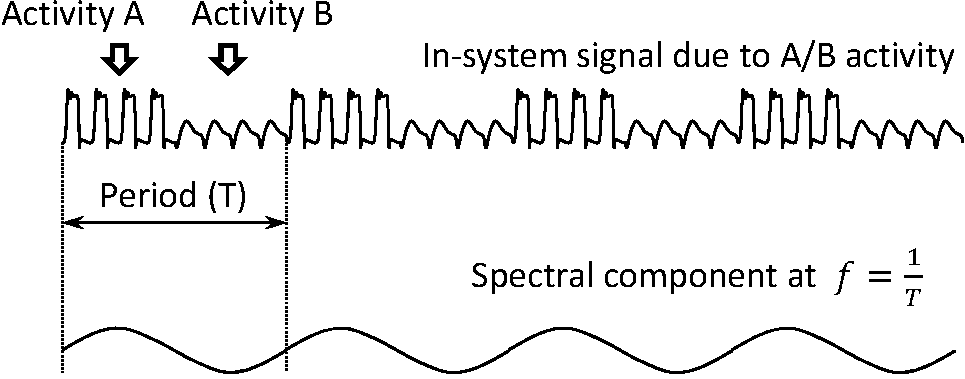
\includegraphics[scale=0.45,clip]{../TEMC_SAVAT/TEMC_314_2013_Fig1a.pdf}
  \caption{The A/B alternation pseudo-code induces emanations at a specific radio frequency by alternating half-periods of A and B activity.}
  \label{Fig:Carrier}
\end{figure}

To generate different cache behavior during load and store instructions, our code (in lines \ref{UpdAddrA} and \ref{UpdAddrB}) updates the address of the accessed memory location so the memory access repeatedly sweeps over an array of appropriate size (fits in L1 cache, does not fit in L1 but fits in L2 cache, or does not fit in L2) to create the desired cache hit/miss behavior. Note that \texttt{ptr1}, \texttt{ptr2}, and \texttt{offset} must be chosen so that the A and B instructions access separate groups of cache blocks to create the desired cache behavior (e.g. every A is a L1 cache hit and every B is a L2 cache hit). Aside from the test instructions (line \ref{TestInstA} for A and line \ref{TestInstB} for B), the executed code should be identical for all instructions/events, so this pointer-update code is present even when the A and/or B instruction is a non-memory instruction (e.g. ADD). Our actual code is written in x86 assembler to minimize the amount of non-under-test activity and prevent compiler optimizations that might make the non-under-test code differ for different under-test instructions (e.g. different instruction scheduling by the compiler, dead code elimination of memory address updates for non-memory instructions, etc.).

Measuring SAVAT using this methodology overcomes several measurement problems. First, the measured signal represents the accumulation of many repetitions of the A/B difference, so this signal can be measured with less sensitive instruments. Second, the difference between A and B side-channel SAVAT is directly measured, avoiding the relative error introduced when measuring A and B signals separately. Finally, the signal is measured at the alternation frequency, which can be adjusted in software by changing the number of A and B instructions per iteration of the alternation loop, resulting in a lower measurement frequency which is within the measurement range of commercially available instruments. We also have the freedom to select a frequency with the least interference from noise and unrelated signals. This is particularly important for the EM emanations side-channel because EM probes pick up numerous unrelated noise sources and radio signals.
